\subsection{Introduction}

The objective is to create a Fuzzy Inference System (FIS) capable of controlling the variation of the Computing Load Percentage (CLPVariation), given some system parameters as input (such as memory, processor, network, etc...).
It is assumed that when the device is operating as a pure Edge device (i.e., CLP
= 0), only networking duties (including routing data to the cloud) are performed.

\subsection{Architecture and Decisions}
% Include all the membership functions, linguistic terms, and rules. Illustrative graphics are encouraged

To help construct the fuzzy system, we have the following system features:
\begin{itemize}
    \item Memory Usage
    \item Processor Load
    \item Input network throughput
    \item Output network throughput
    \item Available output bandwidth
    \item Latency
\end{itemize}
Each feature is a one-minute average, and for each one, the variation rate is also available.

\subsection{Variables}

Because Fuzzy systems' rule base size increases exponentially with the number of inputs, we began by selecting the important features of the system to use, and also how to combine/group them in smaller fuzzy systems.

We decided not to use the Variation values, as it would overcomplicate the system, and the insights that we would get from them would not be very useful. For example, it was hypothesized to group the Processor Load and its Variation, considering that a positive variation for a "long" period of time would mean a high load on the device and the CLP should decrease. However, we do not have a way to record the state, and knowing the current state of the processor load of the device is enough, as we want to keep its usage around a certain value (70\%-80\%).

Because the \textit{Memory Usage} and \textit{Processor Load} are a good indicative of the current performance of the system, and since either of them having extremely high usage will have a great impact on the device performance, we joined these two features to be the inputs of a fuzzy system (FS\_HDR) that have as output \textit{Hardware Resources}.

On the same train of thought, we tried to combine the network features (\textit{Output Throughput, Available Output Bandwidth, Input Throughput} and \textit{Latency}) on a fuzzy system whose output was \textit{Network Usage}, to have an idea of how congested the network could be.

Finally, we computed the value for the CLP based on the \textit{Hardware Resources} and \textit{Network Usage}.

The original architecture is presented in figure \ref{fig:originalFS}.

\begin{figure}[!htb]
    \centering
    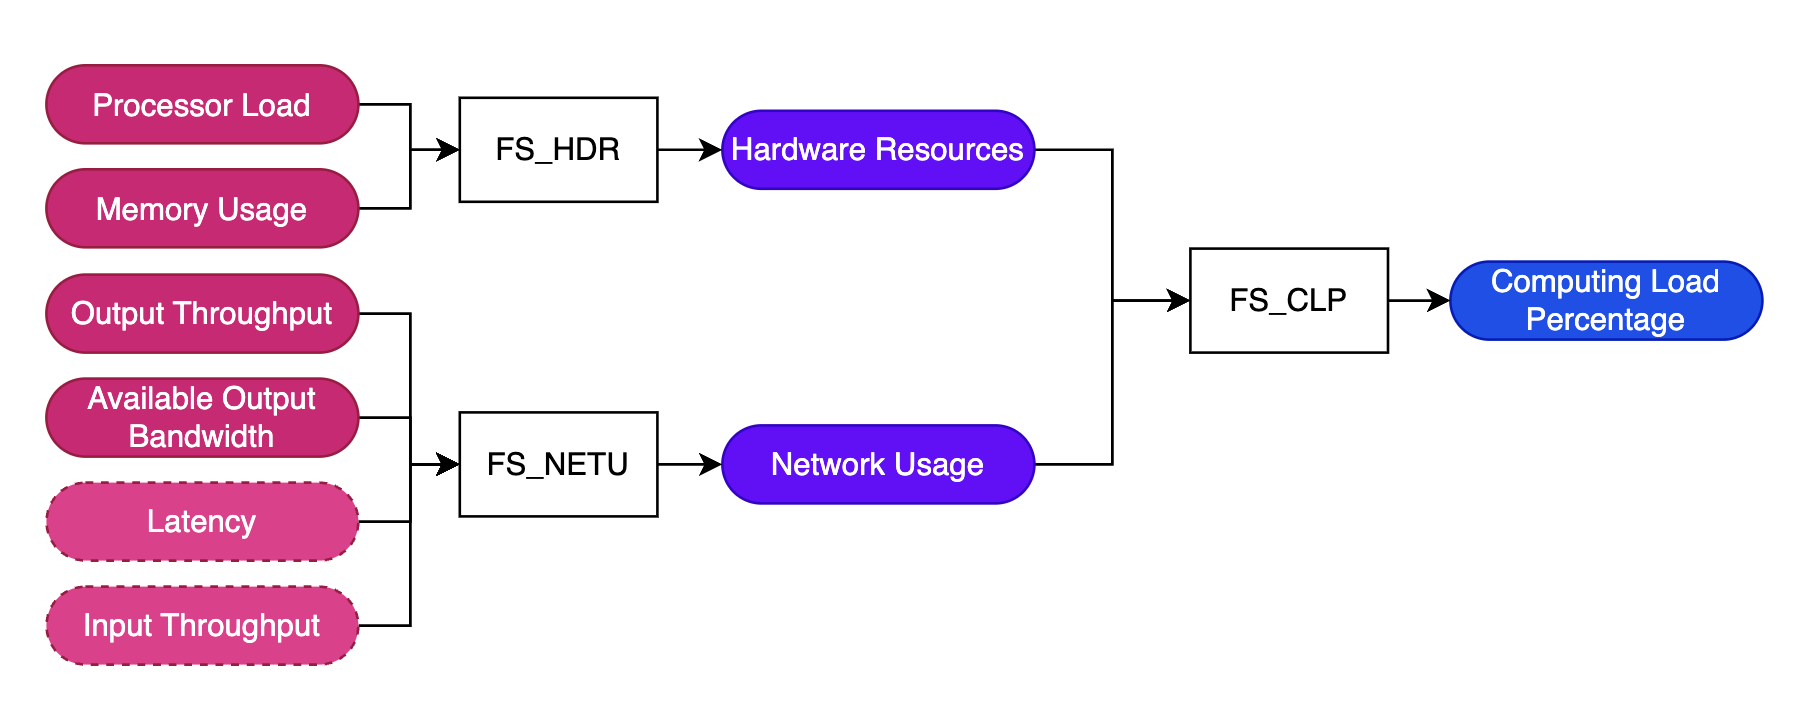
\includegraphics[width=\textwidth, height=\textheight, keepaspectratio]{images/fuzzy_systems_og.png}
    \caption{Original Fuzzy systems architecture}
    \label{fig:originalFS}
\end{figure}

We experimented with combining the features of the \textit{Network Usage} and reached the following conclusions:
\begin{itemize}
    \item Because the input network and the output network are not necessarily correlated, we shouldn't join them in an "outer" fuzzy system, but instead consider the \textit{Input Throughput} in the final Fuzzy System (the one that computes the CLP), as a "tiebreaker" of Hardware and Network load, as high \textit{Input Throughput} implies more data to be processed - and thus an incentive to process it locally. However, while constructing the FAM (Fuzzy Associative Memory) for it, we concluded that its weight was meaningless, and discarded it.
    \item \textit{Latency} was discarded from the \textit{Network Usage}, considering that the packets should reach their destination anyway with high latency, but a congested link will mean loss of packets, and that is worse than a slow link. However, the values that we were getting for the CLP value when considering the \textit{Latency} as an input of the final fuzzy system were not satisfactory, and decided to discard it as well.
\end{itemize}

In the end, we ended up with a fuzzy system that computes the \textit{Output Congestion} (FS\_OUTC), using as input the \textit{Output Throughput} and \textit{Available Output Bandwidth}.
The value for the CLP is then based on the \textit{Hardware Resources} and \textit{Output Congestion}.

The final architecture of the project is presented in figure \ref{fig:finalFS}.

\begin{figure}[!htb]
    \centering
    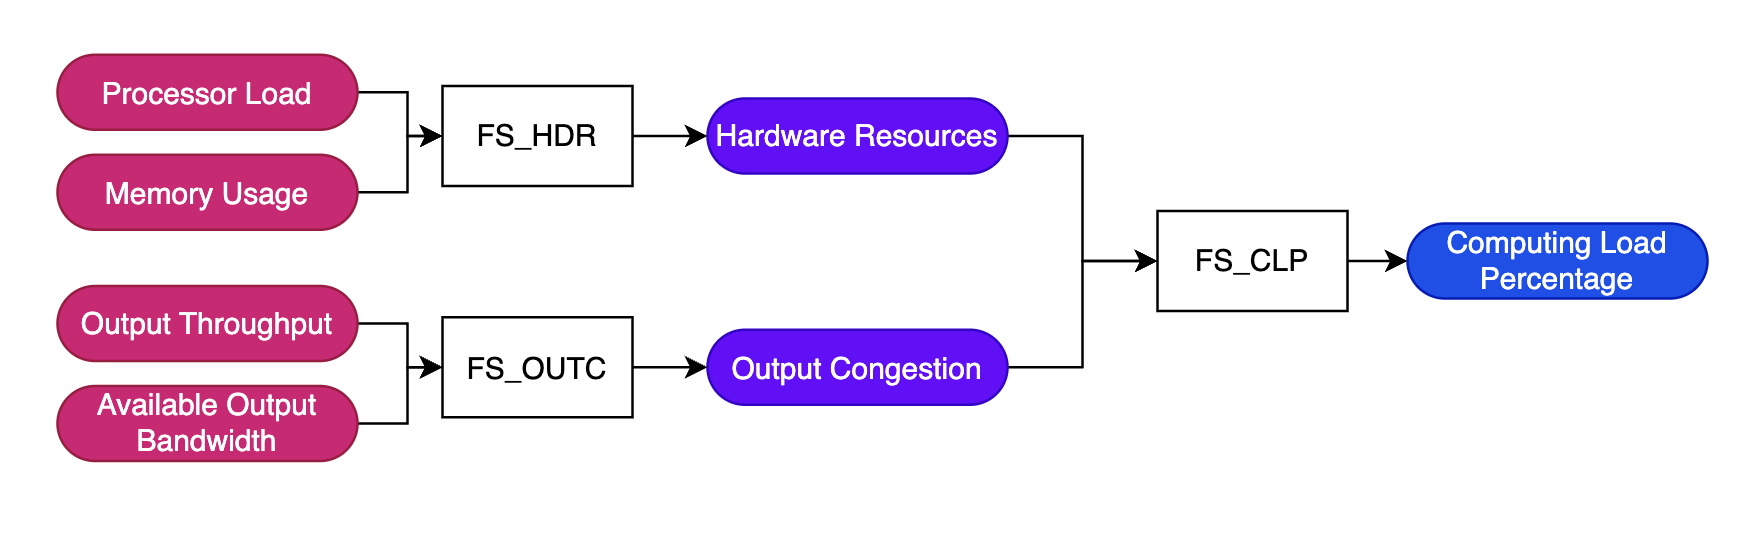
\includegraphics[width=\textwidth, height=\textheight, keepaspectratio]{images/fuzzy_systems_final.png}
    \caption{Final Fuzzy systems architecture}
    \label{fig:finalFS}
\end{figure}


\subsubsection{Linguistic Terms \& Membership Functions (Fuzzy Sets)}
We chose the Linguistic Terms "High", "Medium" and "Low" for all the input Fuzzy Sets, and "Increase", "Maintain" and "Decreased" for the output \textit{CLP Variation}, and to allow a better categorization of the fuzzy sets, we decided to use trapezoids over triangles.
After testing the fuzzy systems, it was necessary to add more members to some fuzzy systems, as shown in the membership functions below (for example, adding a "very high" member to the \textit{Processor Load}, or adding "decrease much" and "increase much" members to the \textit{CLP Variation}).

The Membership Functions for our fuzzy systems are presented in the figures \ref{fig:FS_HDR_FSETS}, \ref{fig:FS_OUTC_FSETS} and \ref{fig:FS_CLP_FSETS}.

\begin{figure}[!htb]
    \centering
    \hspace*{-1cm}
    
    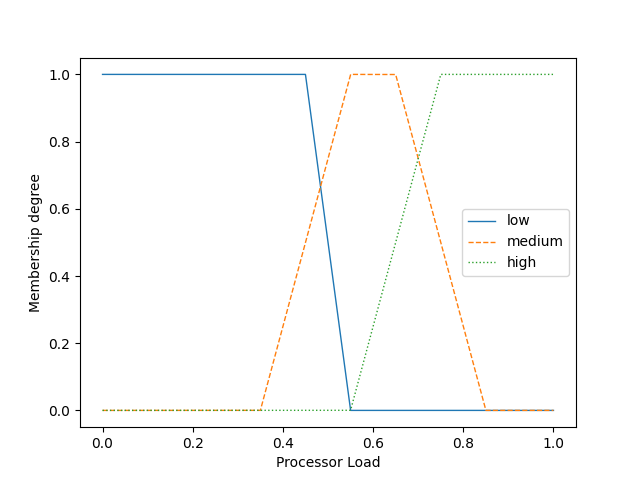
\includegraphics[width=.33\textwidth]{images/plots/ProcessorLoad.png}\hfill
    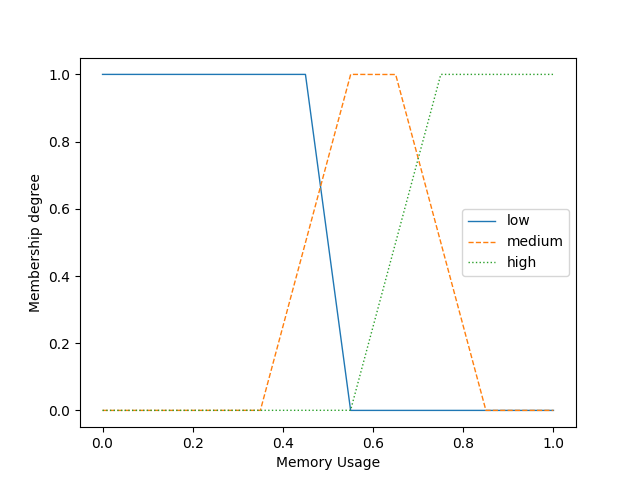
\includegraphics[width=.33\textwidth]{images/plots/MemoryUsage.png}\hfill
    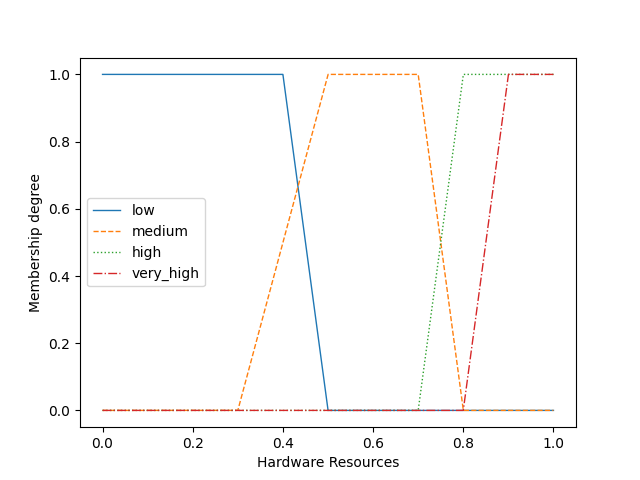
\includegraphics[width=.33\textwidth]{images/plots/CpuMemCLP.png}

    \hspace*{-1cm}
    \caption{Membership functions for the "Hardware Resources" Fuzzy System}
    \label{fig:FS_HDR_FSETS}
\end{figure}

\begin{figure}[!htb]
    \centering
    \hspace*{-1cm}
    
    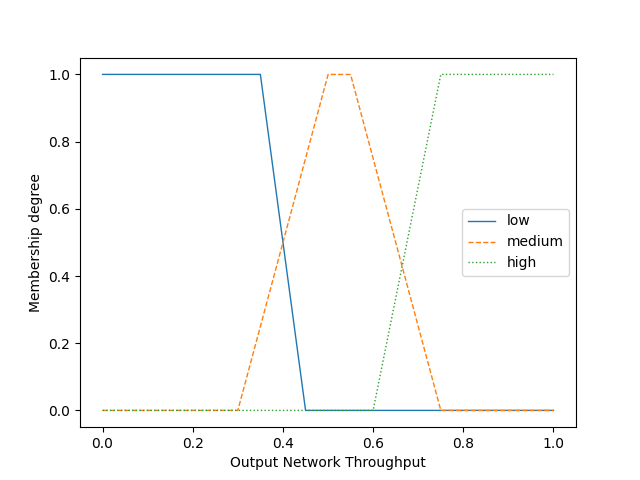
\includegraphics[width=.33\textwidth]{images/plots/OutNetThroughput.png}\hfill
    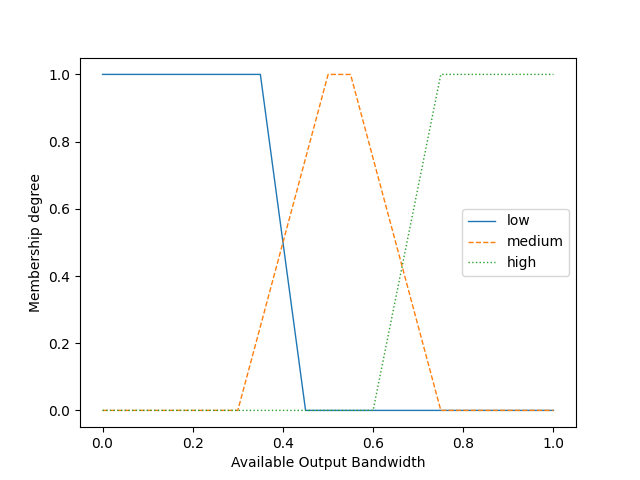
\includegraphics[width=.33\textwidth]{images/plots/AvailOutBandwidth.png}\hfill
    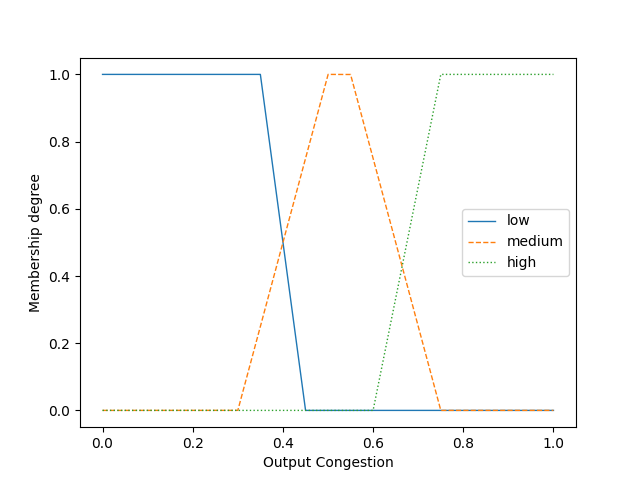
\includegraphics[width=.33\textwidth]{images/plots/OutCongestion.png}
    
    \hspace*{-1cm}
    \caption{Membership functions for the "Output Congestion" Fuzzy System}
    \label{fig:FS_OUTC_FSETS}
\end{figure}

\begin{figure}[!htb]
    \centering
    \hspace*{-1cm}
    
    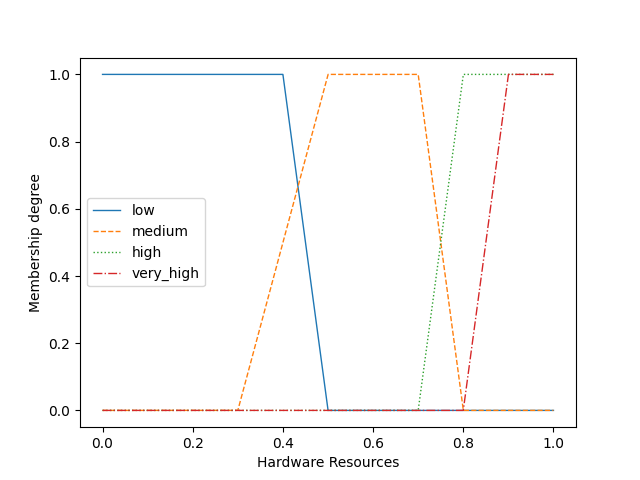
\includegraphics[width=.33\textwidth]{images/plots/CpuMem.png}\hfill
    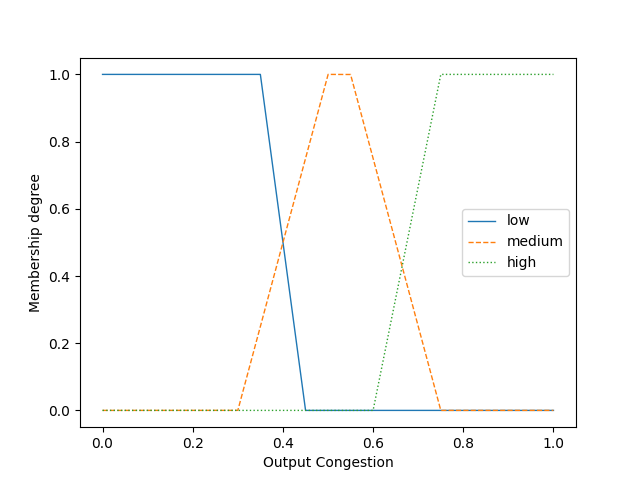
\includegraphics[width=.33\textwidth]{images/plots/OutCongestion.png}\hfill
    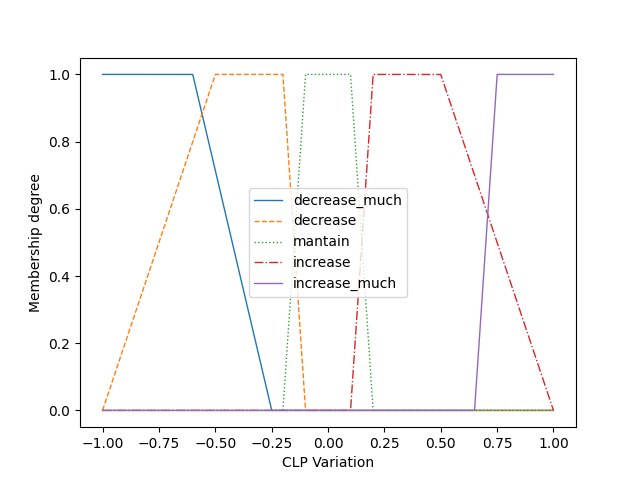
\includegraphics[width=.33\textwidth]{images/plots/CLP.png}
    
    \hspace*{-1cm}
    \caption{Membership functions for the "CLP Variation" Fuzzy System}
    \label{fig:FS_CLP_FSETS}
\end{figure}


\subsubsection{Fuzzy Rules}
Because the output of our final Fuzzy System is a Fuzzy Set, we decided to use a Mamdani Fuzzy Model, with the fuzzy rules shown in the FAMs \ref{tab:FAM_HDR}, \ref{tab:FAM_OUTC} and \ref{tab:FAM_CLP}.
\begin{itemize}
    \item \textbf{Hardware Resources Fuzzy System}
    \begin{table}[!htb]
        \begin{center}
            \begin{tabular}{ |c|c|c|c|c| }
                \hline
                & & \multicolumn{3}{c|}{Processor Load} \\
                \hline
                \multirow{4}{4em}{Memory} 
                &        & Low   & Medium & High \\ 
                & Low    & L     & M      & H \\ 
                & Medium & M     & M      & H \\ 
                & High   & H     & H      & H \\ 
                \hline
            \end{tabular}
            \caption{FAM for Hardware Resources Fuzzy Rules}
            \label{tab:FAM_HDR}
        \end{center}
    \end{table}
    
    \item \textbf{Output Congestion Fuzzy System}
    \begin{table}[!htb]
        \begin{center}
            \begin{tabular}{ |c|c|c|c|c| }
                \hline
                & & \multicolumn{3}{c|}{Output Bandwidth Available} \\
                \hline
                \multirow{4}{4em}{Network Throughput} 
                &        & Low   & Medium & High \\ 
                & Low    & M     & L      & L    \\ 
                & Medium & H     & M      & M    \\ 
                & High   & H     & H      & H    \\ 
                \hline
            \end{tabular}
            \caption{FAM for Output Congestion Fuzzy Rules}
            \label{tab:FAM_OUTC}
        \end{center}
    \end{table}
    
    \item \textbf{CLP Variation Fuzzy System}
    \begin{table}[!htb]
        \begin{center}
            \begin{tabular}{ |c|c|c|c|c| }
                \hline
                & & \multicolumn{3}{c|}{Output Congestion} \\
                \hline
                \multirow{5}{6em}{Hardware Resources} 
                &             & Low   & Medium & High \\ 
                & Low         & ↑↑    & ↑↑     & ↑↑    \\ 
                & Medium      & 0     & ↑      & ↓    \\ 
                & High        & ↓↓    & ↓      & ↓    \\ 
                & Very High   & ↓↓    & ↓↓     & ↓↓   \\
                \hline
            \end{tabular}
            \caption{FAM for CLP Variation Fuzzy Rules}
            \label{tab:FAM_CLP}
        \end{center}
    \end{table}
\end{itemize}


In figures \ref{fig:FS_CpuMem_OUT}, \ref{fig:FS_OutCongestion_OUT} and \ref{fig:FS_CLP_OUT} are the surfaces induced by the rules for the 3 considered fuzzy systems.

\begin{figure}[!htb]
    \centering
    
    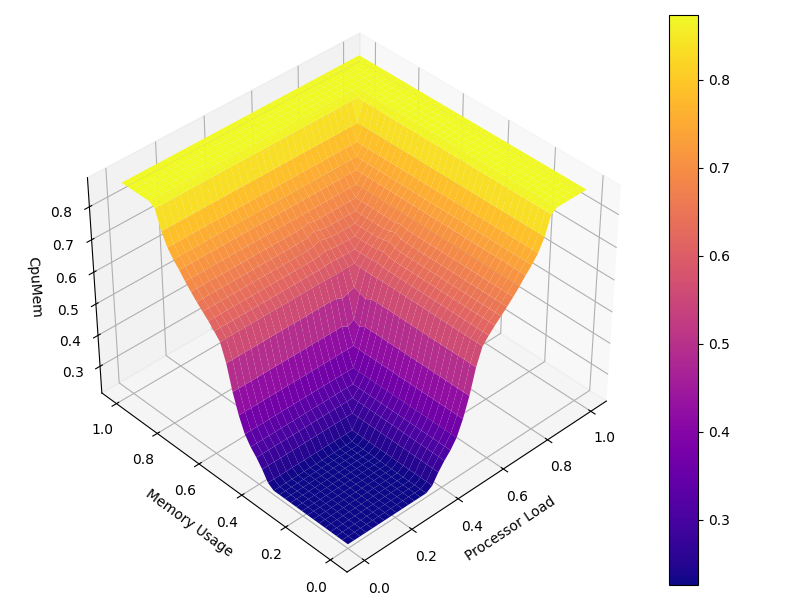
\includegraphics[width=.6\textwidth]{images/plots/CpuMem3D_better.png}\hfill

    \caption{Surface induced by the Hardware Resources Fuzzy System}
    \label{fig:FS_CpuMem_OUT}
\end{figure}

\begin{figure}[!htb]
    \centering
    
    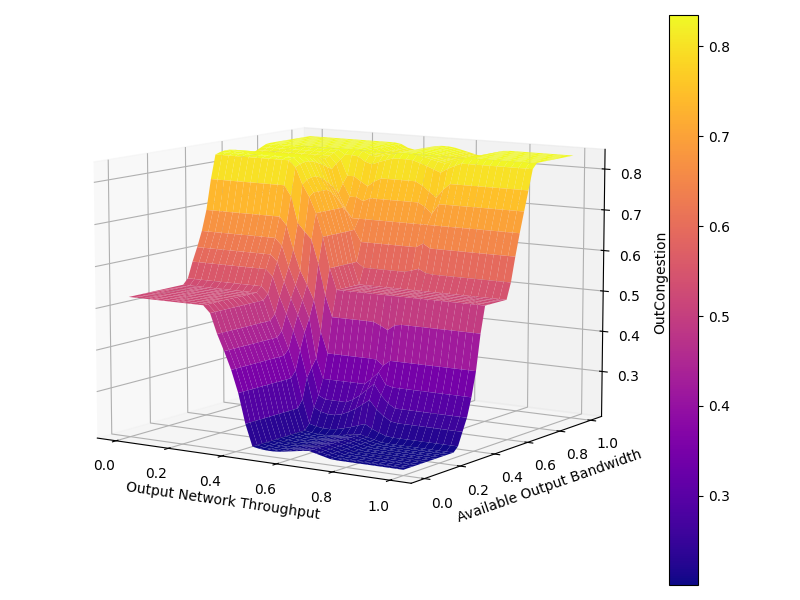
\includegraphics[width=.6\textwidth]{images/plots/OutCongestion3D.png}\hfill
    
    \caption{Surface induced by the  Output Congestion Fuzzy System}
    \label{fig:FS_OutCongestion_OUT}
\end{figure}

\begin{figure}[!htb]
    \centering
    
    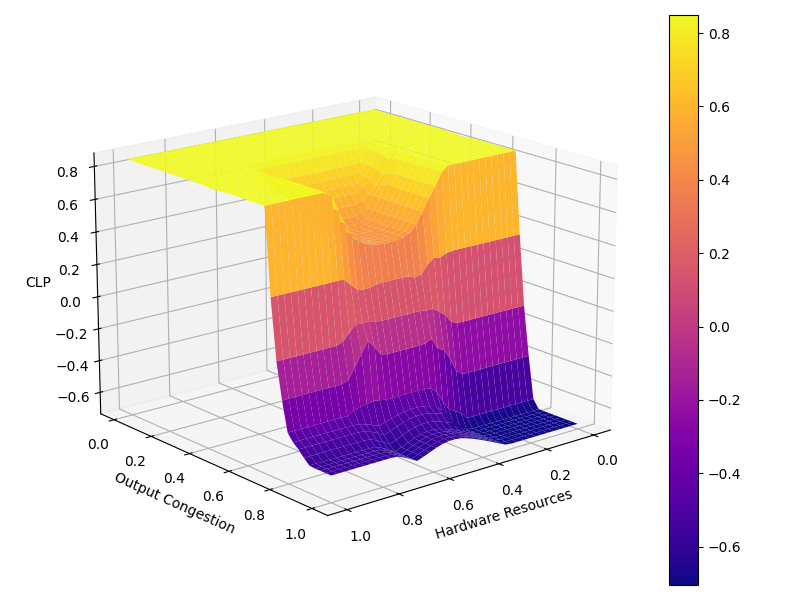
\includegraphics[width=.6\textwidth]{images/plots/CLP3D_better.png}\hfill
    
    \caption{Surface induced by the Computing Load Variation Fuzzy System}
    \label{fig:FS_CLP_OUT}
\end{figure}


\subsection{Testing and Results}

In refining our fuzzy system, we implemented several strategic adjustments to enhance its performance. Firstly, we meticulously modified the rule set to match better our anticipated output, ensuring a more precise correspondence between input variables and system responses. Additionally, we meticulously fine-tuned the trapezoid points, strategically adjusting them to optimize the system's accuracy and efficacy in generating outputs. As a direct outcome of these refinements, we observed a notable improvement in the system's overall performance. However, it's worth noting a particular consequence of these enhancements: our parameter "decrease much" has now a minimum of at -0.6. Even though the rules are effectively being applied as intended, this intrinsic limitation implies that our system's \textit{CLP Variation} cannot extend beyond this threshold.

For the dataset provided, we obtained the results in table \ref{tab:RESULTS_CLP}.
\begin{table}[H]
    \begin{center}
        \begin{tabular}{ |c|c| }
            \hline
            Predicted & Expected \\
            \hline
            84\% & 85\% \\
            85\% & 85\% \\
            85\% & 80\% \\
            81\% & 73\% \\
            59\% & 50\% \\
            52\% & 12\% \\
            -48\% & -31\% \\
            -48\% & -65\% \\
            -54\% & -82\% \\
            -54\% & -85\% \\
            \hline
        \end{tabular}
        \caption{Predicted vs Expected \textit{CLP Variation}}
        \label{tab:RESULTS_CLP}
    \end{center}
\end{table}

As we can see in Table \ref{tab:RESULTS_CLP}, the last 2 lines of the table have a big discrepancy because our system cannot output values below -0.6. The only line that requires more attention is the \nth{6}, where our output is 52\% and the expected value is 12\%. After analyzing the data, we concluded that with the variables we chose to use for our system, we are unable to provide a different output. Only a system with more inputs could produce a closer output to the expected values.
